\documentclass[a4paper]{article}

\def\npart {UD BMEG 671}
\def\nterm {Module 1}
\def\nyear {2026}
\def\nlecturer {Islam and Zurakowski; DiStefano; current modeling guidance}
\def\ncourse {Module 1: Compartmental Modeling Foundations}
\def\ncoursehead {Compartmental Modeling}
\def\nauthor {NanFangHong}

\RequirePackage{etex}
\makeatletter
\ifx \npart \undefined
  \def\npart{PK/PD Notes}
\fi
\ifx \nterm \undefined
  \def\nterm{Reading notes}
\fi
\ifx \nyear \undefined
  \def\nyear{\the\year}
\fi
\ifx \nlecturer \undefined
  \def\nlecturer{the source literature}
\fi
\ifx \nauthor \undefined
  \def\nauthor{NanFangHong}
\fi
\ifx \ncourse \undefined
  \def\ncourse{Pharmacology Reading Note}
\fi
\ifx \ncoursehead \undefined
  \def\ncoursehead{\ncourse}
\fi

\author{Based on \nlecturer \\\small Notes taken by \nauthor}
\date{\nterm\ \nyear}
\title{\npart\ --- \ncourse}

\usepackage{amsfonts}
\usepackage{amsmath}
\usepackage{amssymb}
\usepackage{amsthm}
\usepackage{booktabs}
\usepackage{caption}
\usepackage{enumitem}
\usepackage{fancyhdr}
\usepackage{fontspec}
\usepackage{graphicx}
\usepackage{iftex}
\usepackage{mathtools}
\usepackage{microtype}
\usepackage{siunitx}
\usepackage{tabularx}
\usepackage{tikz}
\usepackage{xcolor}
\usepackage{xurl}
\usepackage{xeCJK}

\IfFontExistsTF{Latin Modern Roman}{
  \setmainfont[Ligatures=NoCommon]{Latin Modern Roman}
}{}

\IfFontExistsTF{Noto Serif CJK SC}{
  \setCJKmainfont{Noto Serif CJK SC}
}{
  \IfFontExistsTF{Songti SC}{
    \setCJKmainfont{Songti SC}
  }{
    \IfFontExistsTF{PingFang SC}{
      \setCJKmainfont{PingFang SC}
    }{}
  }
}

\usepackage[hidelinks,unicode,breaklinks=true]{hyperref}
\hypersetup{
  pdfauthor={\nauthor},
  pdfsubject={\npart\ - \ncourse},
  pdftitle={\npart\ - \ncourse},
  pdfkeywords={PK PD pharmacology reading notes \ncourse}
}

\pagestyle{fancyplain}
\lhead{\emph{\nouppercase{\leftmark}}}
\rhead{
  \ifnum\thepage=1
  \else
    \npart\ \ncoursehead
  \fi}

\theoremstyle{definition}
\newtheorem*{aim}{Aim}
\newtheorem*{assumption}{Assumption}
\newtheorem*{defi}{Definition}
\newtheorem*{eg}{Example}
\newtheorem*{notation}{Notation}
\newtheorem*{question}{Question}
\newtheorem*{remark}{Remark}
\newtheorem*{warning}{Warning}

\theoremstyle{plain}
\newtheorem{nthm}{Theorem}[section]
\newtheorem{nprop}[nthm]{Proposition}

\renewcommand{\labelitemi}{--}
\renewcommand{\labelitemii}{$\circ$}
\renewcommand{\labelenumi}{(\roman{*})}

\let\stdsection\section
\renewcommand\section{\newpage\stdsection}

\newcommand{\dd}{\mathop{}\!\mathrm{d}}
\newcommand{\Emax}{E_{\max}}
\newcommand{\pksym}[1]{\ifmmode\text{\textit{#1}}\else\textit{#1}\fi}
\newcommand{\pklab}[1]{\mathrm{#1}}
\newcommand{\ECfifty}{\pksym{EC}_{50}}
\newcommand{\term}[1]{\emph{#1}}
\makeatother

\title{UD BMEG 671 Module 1 --- Compartmental\\ Modeling Foundations}
\author{Based on BMEG/ELEG 471/671 lectures\\\small DiStefano and current modeling guidance\\\small Notes taken by NanFangHong}
\usetikzlibrary{arrows.meta,positioning,calc,shapes.geometric,decorations.pathreplacing,fit}
\emergencystretch=4em
\sloppy
\captionsetup{width=0.9\textwidth, justification=raggedright, singlelinecheck=false}
\lhead{\emph{\npart}}
\rhead{\ncoursehead}

\DeclareMathOperator{\rank}{rank}
\DeclareMathOperator{\diag}{diag}
\DeclareMathOperator{\spanop}{span}
\newcommand{\R}{\mathbb{R}}
\newcommand{\ddt}{\frac{\dd}{\dd t}}
\newcommand{\vect}[1]{\boldsymbol{#1}}
\newcommand{\mat}[1]{\mathbf{#1}}
\newcommand{\state}[1]{\mathsf{#1}}
\newcommand{\param}[1]{\theta_{\mathrm{#1}}}
\newcommand{\given}{\,|\,}
\newcommand{\Prob}{\mathbb{P}}
\newcommand{\Ex}{\mathbb{E}}
\newcommand{\Normal}{\mathcal{N}}
\newcommand{\data}{\mathcal{D}}
\newcommand{\CL}{\ensuremath{\pksym{CL}}}
\newcommand{\Vd}{\ensuremath{\pksym{V}_d}}
\newcommand{\PK}{\ensuremath{\pksym{PK}}}
\newcommand{\PD}{\ensuremath{\pksym{PD}}}
\newcommand{\PKPD}{\ensuremath{\pksym{PK}/\pksym{PD}}}
\newcommand{\QSP}{\ensuremath{\pksym{QSP}}}
\newcommand{\PBPK}{\ensuremath{\pksym{PBPK}}}
\newcommand{\MIDD}{\ensuremath{\pksym{MIDD}}}
\newcommand{\SBML}{\ensuremath{\pksym{SBML}}}
\newcommand{\MATLAB}{\ensuremath{\pksym{MATLAB}}}
\newcommand{\SimBio}{\ensuremath{\pksym{SimBiology}}}
\newcommand{\IRate}{\ensuremath{\pksym{IR}}}
\newcommand{\qin}{q_{\mathrm{in}}}
\newcommand{\qout}{q_{\mathrm{out}}}
\newcommand{\qone}{q_1}
\newcommand{\qtwo}{q_2}
\newcommand{\Bone}{B_{\mathrm{bone}}}
\newcommand{\Bint}{B_1}
\newcommand{\Bblood}{B_2}
\newcommand{\unitstep}{\mathbf{1}(t)}
\newcommand{\dirac}{\delta(t)}
\newcommand{\code}[1]{\texttt{\detokenize{#1}}}

\definecolor{bmegblue}{HTML}{114B7A}
\definecolor{bmegteal}{HTML}{178F88}
\definecolor{bmeggreen}{HTML}{4E8F4A}
\definecolor{bmegpurple}{HTML}{6651A6}
\definecolor{bmegred}{HTML}{B94444}
\definecolor{bmegorange}{HTML}{C77A2B}
\definecolor{bmeglight}{HTML}{F3F6F7}
\tikzset{
  comp/.style={draw=bmegblue!75, fill=bmeglight, rounded corners=2pt, align=center, inner sep=5pt, minimum width=25mm, minimum height=9mm},
  species/.style={draw=bmegpurple!75, fill=bmeglight, rounded corners=2pt, align=center, inner sep=5pt, minimum width=22mm, minimum height=9mm},
  flow/.style={-{Stealth[length=2.2mm]}, thick, draw=bmegblue!90},
  loss/.style={-{Stealth[length=2.2mm]}, thick, draw=bmegred!90},
  info/.style={font=\footnotesize, align=center}
}

\begin{document}
\maketitle
{\small
  \noindent\textbf{Reading motive}\\
  这是 UD BMEG/ELEG 471/671 前三次课的学习笔记。课程标题叫 Advanced Biomedical and Pharmaceutical Modeling，但前三节课真正搭的是一门语言：怎样把生物医学故事翻译成 compartments, states, inputs, outputs, rates, ODEs, code, and validation。我的目标不是逐页复述课件，而是把课堂 transcript、带标注和无标注 lecture notes、\MATLAB{} live scripts、DiStefano 的 dynamic systems biology 视角、以及 2026 年仍在更新的 \MIDD{}/model credibility 语境接成一个能自学的开端。\par\hfill[course note]

  \vspace{5pt}
  \noindent\textbf{Reader}\\
  假设读者已经见过一点微积分和线性代数，但还没有真正把 ODE、系统、药物动力学、疾病动力学、代码验证和数据拟合放在同一个脑图里。这里会慢一点，把每个符号先问清楚：它是 amount, concentration, rate constant, input, output, measurement, decision variable, or hidden biological state?\par\hfill[from zero]

  \vspace{5pt}
  \noindent\textbf{Update}\\
  课程材料来自 Fall 2025。本笔记保留 Islam/Zurakowski 的课堂主线，同时补入 FDA \MIDD{} paired meeting program, ICH M15, ASME V\&V 40, \SBML{}, and \SimBio{} 的当前语境：模型不只是 homework equation，而是可能进入 regulatory reasoning、model exchange、credibility assessment 和 therapeutic decision 的科学对象。\par\hfill[2026 view]
}

\tableofcontents

\section{The Course Spine}

\subsection{What the first three lectures are really doing}

The syllabus says the course will cover compartmental network diagrams, linear systems theory, controllability, observability, reachability, detectability, nonlinear interactions, stability, identifiability, sensitivity analysis, likelihood functions, parameter estimation, uncertainty, Markov chain Monte Carlo, model selection, and statistical evaluation of fitted models \cite{bmeg671Syllabus2025}. That sounds like many topics. The first three lectures reveal the hidden spine:
\[
  \begin{aligned}
  \text{diagram}
  &\longrightarrow
  \text{mass balance}
  \longrightarrow
  \text{ODE}\\
  &\longrightarrow
  \text{simulation}
  \longrightarrow
  \text{data comparison}
  \longrightarrow
  \text{decision}.
  \end{aligned}
\]

This is the same grammar that later appears under many names:
\begin{itemize}[leftmargin=2em]
  \item in pharmacokinetics: dose \(\to\) concentration \(\to\) exposure \(\to\) response;
  \item in systems biology: reaction network \(\to\) state equations \(\to\) pathway dynamics;
  \item in control theory: state \(\to\) input \(\to\) output \(\to\) observability and controllability;
  \item in inference: latent state \(\to\) measurement model \(\to\) likelihood \(\to\) uncertainty;
  \item in model credibility: question of interest \(\to\) model use \(\to\) verification and validation evidence.
\end{itemize}

So the first three lectures are not merely ``how to write a one-compartment ODE.'' They are a compact version of the whole course: choose a state, write a conservation law, solve or simulate, verify the implementation, validate against a truth source, and then ask whether the model is fit for its intended use.

\subsection{Why this matters in biomedical and pharmaceutical modeling}

Biomedical systems are often observable only through partial, delayed, noisy measurements. We may dose the blood, observe plasma concentration, care about a tissue target, and make a clinical decision about efficacy or toxicity. The thing we want is rarely the thing we directly measure.

Compartmental modeling is a disciplined compromise. It says: do not try to draw every cell. Instead, choose a small number of states whose changes explain the data and decision. Each state is a storage variable: amount of drug in blood, amount of metabolite in urine, number of infected individuals, abundance of a signaling species, mass of butyrate in gut, or active osteoblast population.

The course begins here because every later method depends on this first act of abstraction. If the state variables are ill-chosen, no algorithm can rescue the model. If the units are inconsistent, the simulation may be beautiful but meaningless. If the output equation does not correspond to the measurement, parameter estimation will learn the wrong thing.

\subsection{The DiStefano perspective}

DiStefano's textbook frames dynamic systems biology as modeling and simulation of systems whose variables change in time \cite{distefano2015DynamicSystemsBiology}. The key word is dynamic. A static regression might say that high concentration correlates with high effect. A dynamic model asks how concentration becomes high, when it becomes high, why it decays, and what hidden rates control that time course.

For this course, the useful mental model is:
\[
  \begin{aligned}
  \boxed{\text{biological story}}
  &\stackrel{\text{state choice}}{\longrightarrow}
  \boxed{\dot{\vect q}=f(\vect q,\vect u,\vect\theta,t)}\\
  &\stackrel{\text{output map}}{\longrightarrow}
  \boxed{\vect y=g(\vect q,\vect\theta,t)}.
  \end{aligned}
\]
The story is qualitative. The ODE is quantitative. The output map is what makes it testable.

\section{The Compartmental Grammar}

\subsection{Compartment, species, state, and output}

A compartment is not merely a box in a diagram. In Lecture 1, the working definition is a physical or conceptual space in which the quantity of interest is treated as homogeneously distributed, with mixing inside the compartment faster than transfer between compartments \cite{bmeg671Lecture1Slides2025,bmeg671TranscriptAug272025}. The word ``treated'' matters. A compartment is a modeling decision, not a claim that nature literally contains boxes.

We need four related but distinct objects:
\begin{itemize}[leftmargin=2em]
  \item A \term{compartment} is the location or pool: blood, urine, gut, bone, susceptible population, infected population.
  \item A \term{species} is what is counted: parent drug, metabolite, T4, T3, butyrate, infected individuals.
  \item A \term{state variable} is the time-varying amount or concentration represented in the model: \(q(t)\), \(C(t)\), \(S(t)\), \(I(t)\), \(R(t)\).
  \item An \term{output} is what the experiment reports: a plasma concentration, urinary amount, biomarker, imaging measurement, viral load, or clinical score.
\end{itemize}

The trap is to collapse all four into one word. In a simple drug model, blood may be the compartment, parent drug the species, \(q_{\mathrm{blood}}(t)\) the state, and measured plasma concentration \(C_p(t)=q_{\mathrm{blood}}(t)/V_p\) the output. If the experiment measures urine, the output is not the central amount; it is a different state or a derived cumulative excretion.

\subsection{Same compartment, different species}

The transcript uses the thyroid example to show that a compartment need not correspond one-to-one to a state. T4 and T3 can both exist inside a cell. The physical space is the same, but the species differ, so the model needs two state variables:
\[
  q_{\mathrm{T4,cell}}(t),\qquad q_{\mathrm{T3,cell}}(t).
\]
If T4 is converted to T3, the arrow is not a movement between physical rooms. It is a reaction between species within a location. In a diagram, both movement and reaction may look like arrows, but their interpretation differs.

\begin{center}
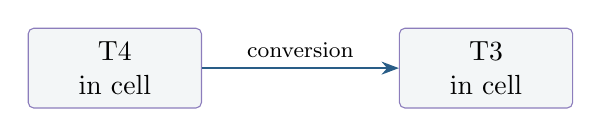
\begin{tikzpicture}[node distance=25mm]
  \node[species] (t4) {T4\\in cell};
  \node[species, right=of t4] (t3) {T3\\in cell};
  \draw[flow] (t4) -- node[above,info]{conversion} (t3);
\end{tikzpicture}
\end{center}

This distinction becomes essential in systems biology and \QSP{} because compartments often contain many species. A liver compartment might contain parent drug, metabolite, enzyme, transporter, receptor, and signal. The same physical organ can generate a high-dimensional state vector.

\subsection{Different compartments, same species}

The blood/urine example is the opposite. The species may be the same drug, but the locations differ:
\[
  q_{\mathrm{blood}}(t),\qquad q_{\mathrm{urine}}(t).
\]
If urine amount is cumulative excretion, then the urine state may have no outflow over the sampling window:
\[
  \ddt q_{\mathrm{urine}}(t)=k_{\mathrm{renal}}q_{\mathrm{blood}}(t).
\]
This state is not a storage compartment with reversible exchange; it is an accounting compartment. That is perfectly legitimate, but it changes the interpretation of the arrow.

\subsection{Central and peripheral lumping}

The transcript also gives a pharmacokinetic example: blood and highly perfused organs may be lumped into a central compartment, while slower tissues become peripheral compartments \cite{bmeg671TranscriptAug272025}. The point is not that liver, kidney, lung, brain, and blood are physically one place. The point is that, at the time scale and measurement resolution of the experiment, they may equilibrate quickly relative to other transfers.

\begin{center}
\resizebox{0.92\textwidth}{!}{%
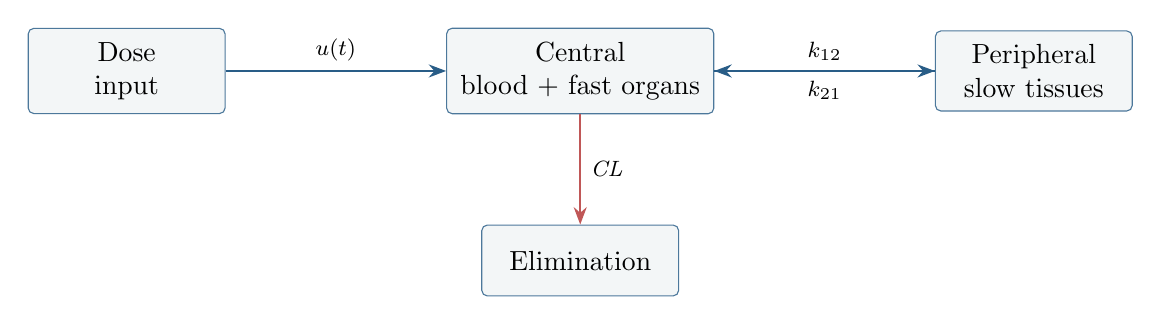
\begin{tikzpicture}[node distance=28mm]
  \node[comp] (dose) {Dose\\input};
  \node[comp, right=of dose] (central) {Central\\blood + fast organs};
  \node[comp, right=of central] (periph) {Peripheral\\slow tissues};
  \node[comp, below=14mm of central] (elim) {Elimination};
  \draw[flow] (dose) -- node[above,info]{\(u(t)\)} (central);
  \draw[flow] (central) -- node[above,info]{\(k_{12}\)} (periph);
  \draw[flow] (periph) -- node[below,info]{\(k_{21}\)} (central);
  \draw[loss] (central) -- node[right,info]{\(\CL\)} (elim);
\end{tikzpicture}
}
\end{center}

Lumping is powerful, but it is also dangerous. It hides spatial detail. A central compartment volume is not a literal anatomical volume; it is an apparent volume compatible with the observed concentration-time curve. A useful rule is:
\begin{center}
\fbox{\parbox{0.86\textwidth}{\centering lump states only when the lost detail is not needed for the question of interest.}}
\end{center}
This phrase anticipates ICH M15: model quality is judged relative to the question the model is meant to answer, not in the abstract \cite{ichM15Midd2026}.

\section{From Diagram to ODE}

\subsection{The mass-balance sentence}

The first mathematical sentence of the course is:
\[
  \text{rate of change inside}
  =
  \text{rate in}
  -
  \text{rate out}
  +
  \text{rate produced}
  -
  \text{rate consumed}.
\]
For a single amount \(q(t)\), this becomes
\[
  \ddt q(t)=\sum \text{inflows}-\sum \text{outflows}.
\]
Everything else is elaboration.

If a first-order loss has rate constant \(k\), the outflow is \(kq(t)\). This is not magic. The units force it:
\[
  [k]=\mathrm{time}^{-1},\qquad [q]=\mathrm{amount},\qquad [kq]=\mathrm{amount}/\mathrm{time}.
\]
In the transcript, the instructor emphasizes a subtle point: dimension is not enough; units must match as well \cite{bmeg671TranscriptAug292025}. A term in kg/s cannot be added directly to kg/hour until it is converted.

\subsection{Sign checking}

Every arrow leaving a state should appear with a minus sign in that state's equation. Every arrow entering a state should appear with a plus sign. If a two-compartment diagram has transfer \(k_{21}\qone\) from state 1 to state 2, then:
\[
  \dot{\qone}\text{ contains }-k_{21}\qone,\qquad
  \dot{\qtwo}\text{ contains }+k_{21}\qone.
\]
This is the simplest verification test. Before running \MATLAB{}, check whether each arrow appears twice, once as a loss and once as a gain, unless it is an external input or external sink.

\subsection{State-space form}

Linear compartmental models can be written as
\[
  \dot{\vect q}(t)=\mat A\vect q(t)+\mat B\vect u(t),
  \qquad
  \vect y(t)=\mat C\vect q(t).
\]
Here \(\vect q\) is the state vector, \(\vect u\) is the input vector, and \(\vect y\) is the output vector. This notation is not merely cosmetic. It is the bridge to the later course topics:
\begin{itemize}[leftmargin=2em]
  \item controllability asks whether inputs can move the state through relevant directions;
  \item observability asks whether outputs contain enough information to reconstruct states;
  \item identifiability asks whether parameters can be inferred from outputs;
  \item stability asks whether trajectories decay, grow, or settle;
  \item sensitivity asks which parameter perturbations change outputs.
\end{itemize}

The first three lectures only touch the edge of these topics, but the notation is already present.

\section{Inputs: Step Versus Impulse}

\subsection{Why inputs deserve their own section}

Inputs are where mathematical idealization meets experimental protocol. An intravenous bolus, a constant infusion, an oral dose, an endogenous production rate, and a viral exposure are all ``inputs,'' but they enter an ODE differently.

The lectures introduce two ideal inputs:
\[
  \unitstep =
  \begin{cases}
    0, & t<0,\\
    1, & t\ge 0,
  \end{cases}
  \qquad
  \dirac.
\]
The unit step turns something on and keeps it on. The Dirac impulse deposits a finite amount at an instant.

\subsection{Bolus as impulse}

The one-compartment bolus model is written as
\[
  \ddt q(t)=Q_0\dirac-kq(t).
\]
The impulse term means that a total amount \(Q_0\) is placed into the system at \(t=0\). For \(t>0\), the equation is simply
\[
  \ddt q(t)=-kq(t),\qquad q(0^+)=Q_0.
\]
This is why the \MATLAB{} live script treats the impulse as an initial condition rather than trying to evaluate a Dirac delta numerically \cite{bmeg671MatlabImpulse2025,bmeg671TranscriptAug292025}.

\subsection{Infusion or production as step}

A constant infusion or endogenous production rate is different:
\[
  \ddt q(t)=\IRate\,\unitstep-kq(t).
\]
For \(t\ge 0\), this is
\[
  \ddt q(t)=\IRate-kq(t).
\]
The input persists at every time. In code, it belongs inside the right-hand-side function, not just in the initial condition.

\subsection{The experimental interpretation}

The same equation can describe different biomedical protocols:
\begin{itemize}[leftmargin=2em]
  \item \(Q_0\dirac\): IV bolus drug dose, instantaneous tracer injection, one-time inoculum.
  \item \(\IRate\unitstep\): constant IV infusion, continuous nutrient supply, zero-order endogenous production, step change in stimulus.
  \item \(u(t)\): arbitrary time-varying dose schedule, pulsatile hormone input, piecewise dosing regimen.
\end{itemize}

The modeler should always write the protocol in words before choosing \(u(t)\). A common beginner error is to choose an input because the equation is familiar, not because it matches the experiment.

\section{One Compartment Impulse}

\subsection{Equation and solution}

For an impulse input at \(t=0\), the post-dose model is
\[
  \ddt q(t)=-kq(t),\qquad q(0)=Q_0.
\]
Separation of variables gives
\[
  q(t)=Q_0e^{-kt}.
\]
The concentration version is obtained by dividing by a volume:
\[
  C(t)=\frac{q(t)}{V}=C_0e^{-kt}.
\]
The half-life is
\[
  t_{1/2}=\frac{\log 2}{k}.
\]
In pharmacokinetics, if \(k=\CL/\Vd\), then
\[
  t_{1/2}=\frac{\log 2\,\Vd}{\CL}.
\]
This formula is a useful preview of later \PK{} notes: half-life is not a primitive mechanism. It is a derived consequence of clearance and volume.

\subsection{What the solution means}

The exponential curve says that the amount lost per unit time is proportional to the amount present. At high amount, loss is fast. At low amount, loss is slow. The system has no finite positive steady state because there is no continuing input:
\[
  q(t)\to 0.
\]

The slope on a semilog plot is \(-k\). This is why first-order elimination is visually recognizable. If data bend away from a straight semilog line, the one-compartment first-order model may be missing absorption, distribution, nonlinear elimination, assay issues, or multiple phases.

\subsection{Code pattern}

The live script's code pattern is conceptually:
\begin{verbatim}
t = 0:0.1:10;
k = 1;
Q0 = 1;
qi = Q0;
soln = ode45(@(t,y) ODEs(t,y), t, qi);
q_sol = deval(soln,t,1);
true_sol = Q0*exp(-k*t);
\end{verbatim}
and the right-hand side is:
\begin{verbatim}
function derivVector = ODEs(t,y)
  k = 1;
  q = y(1);
  dqdt = -k*q;
  derivVector = [dqdt]';
end
\end{verbatim}

This code teaches three habits:
\begin{itemize}[leftmargin=2em]
  \item use an ODE function that takes \(t\) and \(y\), even if \(t\) is not explicitly used;
  \item return a column vector, hence the transpose in \code{[dqdt]'};
  \item compare with an analytical solution when one exists.
\end{itemize}

\subsection{Verification and validation}

The lecture distinguishes verification from validation \cite{bmeg671TranscriptAug292025}. For this example:
\begin{itemize}[leftmargin=2em]
  \item Verification: did the code implement \(\dot q=-kq\) correctly? Does the numerical solution match \(Q_0e^{-kt}\)?
  \item Validation: does this equation describe a real experimental concentration-time curve well enough for the intended question?
\end{itemize}
Analytical comparison verifies numerical implementation. It does not automatically validate biological adequacy.

\section{One Compartment Step}

\subsection{Equation and solution}

For a constant input after time zero:
\[
  \ddt q(t)=\IRate-kq(t),\qquad q(0)=q_0.
\]
The solution is
\[
  q(t)=\frac{\IRate}{k}
  +
  \left(q_0-\frac{\IRate}{k}\right)e^{-kt}.
\]
The steady state is
\[
  q^*=\frac{\IRate}{k}.
\]
This is one of the most important formulas in the first week. It says:
\[
  \text{steady state amount}
  =
  \frac{\text{input rate}}{\text{fractional loss rate}}.
\]

\subsection{Why different initial values converge}

The step live script compares two initial values and shows both trajectories approach the same steady state \cite{bmeg671MatlabStep2025}. That happens because the system is linear and stable. Initial condition controls transient memory; input and loss rate control the eventual equilibrium.

If \(q_0<\IRate/k\), the curve rises. If \(q_0>\IRate/k\), the curve falls. If \(q_0=\IRate/k\), the system is already at steady state. The exponential factor \(e^{-kt}\) is the memory of the initial condition.

\subsection{Drug interpretation}

For an IV infusion with central amount \(q\), concentration \(C=q/V\), and elimination rate constant \(k=\CL/V\):
\[
  C^*=\frac{\IRate}{\CL}.
\]
This is the familiar pharmacokinetic steady-state relationship. Again, the course's simple ODE is already a real drug-development tool: it tells us how a maintenance infusion rate maps to target concentration.

\subsection{Step-input code pattern}

The corresponding live script should be read as a miniature experiment. The input rate is not hidden in the initial condition; it lives inside the right-hand side:
\begin{verbatim}
t = 0:0.1:10;
k = 1;
IR = 1;
qi = 0;
soln = ode45(@(t,y) ODEs(t,y), t, qi);
q_sol = deval(soln,t,1);
q_ss = IR/k;
\end{verbatim}
with
\begin{verbatim}
function derivVector = ODEs(t,y)
  k = 1;
  IR = 1;
  q = y(1);
  dqdt = IR - k*q;
  derivVector = [dqdt]';
end
\end{verbatim}
This tiny difference from the impulse script is the whole modeling lesson. An impulse dose changes \(q(0)\). A sustained infusion changes \(\dot q\) for as long as the infusion is active. If the code and the intended experiment disagree here, every later plot may look smooth and still be answering the wrong question.

\section{The MATLAB Pattern}

\subsection{Why code appears so early}

The lectures put \MATLAB{} in the first week because modeling is not only equation writing. A model becomes operational only when it can be simulated, checked, and compared. In \QSP{}, \PBPK{}, and \PKPD{} workflows, the gap between a diagram and a credible result often lives in code details: units, signs, solver choice, parameter passing, initial conditions, and output extraction.

MathWorks' \SimBio{} tutorials now explicitly frame the tool around \QSP{}, \PBPK{}, and \PKPD{} modeling and analysis \cite{mathworksSimBiologyTutorials2026}. This is exactly why the course asks students to become comfortable with programmatic ODE simulation before using higher-level graphical tools.

\subsection{ODE function shape}

The canonical shape is:
\begin{verbatim}
function derivVector = ODEs(t,y)
  q1 = y(1);
  q2 = y(2);
  dq1dt = ...;
  dq2dt = ...;
  derivVector = [dq1dt,dq2dt]';
end
\end{verbatim}
The solver does not care what the states mean. It receives a vector and returns a derivative vector. The meaning is carried by our naming, equations, and documentation.

\subsection{Parameter passing and reusable code}

The first-week scripts deliberately hard-code simple parameters inside \code{ODEs}. That makes the classroom algebra easy to see. As soon as the same model is scanned over doses, rates, or patient values, the safer habit is to pass parameters through a closure:
\begin{verbatim}
theta = [k, IR];
odeFunc = @(t,y) ODEs(t,y,theta);
soln = ode45(odeFunc, t, qi);

function derivVector = ODEs(t,y,theta)
  k = theta(1);
  IR = theta(2);
  q = y(1);
  dqdt = IR - k*q;
  derivVector = [dqdt]';
end
\end{verbatim}
This is not software decoration. It separates model structure from the experiment being run. Later vaccine and stability scripts use exactly this idea: the ODE function encodes mechanism, while the outer script changes inputs, parameters, initial conditions, or time windows.

\subsection{Impulse versus step in code}

The transcript's distinction is worth making explicit:
\[
  \begin{array}{lll}
  \text{impulse dose} & \Rightarrow & \text{put dose in initial condition},\\
  \text{step input} & \Rightarrow & \text{put rate inside ODE function}.
  \end{array}
\]
If an impulse is coded as a finite input at every time step, the simulation adds too much mass. If a continuous infusion is coded only as an initial condition, the input stops immediately. These are not small coding choices; they change the experiment being simulated.

\subsection{ode45 and ode15s}

The transcript contrasts nonstiff and stiff solvers. In ordinary \MATLAB{} usage, \code{ode45} is a default nonstiff Runge--Kutta solver, while \code{ode15s} is commonly used for stiff systems \cite{bmeg671TranscriptAug292025,bmeg671TranscriptSep032025}. Stiffness often appears when a model has both very fast and very slow processes. Biomedical models frequently do: receptor binding may equilibrate rapidly, while disease progression evolves over weeks.

The beginner lesson is not to memorize solver taxonomy. It is to watch for solver warnings, step-size pathologies, impossible negative concentrations, and sensitivity to tolerances.

\subsection{deval versus array output}

The first live scripts use \code{deval} to evaluate the solution at requested time points. The SIR-style example discussed in transcript also uses the direct array output form from the solver. Both are legitimate. The deeper point is to keep the time vector and output columns aligned:
\[
  \text{column 1}=\text{state 1},\quad
  \text{column 2}=\text{state 2},\quad
  \ldots
\]
Many modeling errors are indexing errors wearing scientific clothing.

\section{Two Compartment Linear Model}

\subsection{Diagram}

Lecture 1 introduces a two-compartment model; Lecture 3 turns it into \MATLAB{} code \cite{bmeg671Lecture1Slides2025,bmeg671Lecture2Slides2025,bmeg671MatlabTwoCompartment2025}. Let \(\qone\) and \(\qtwo\) be amounts in two compartments. Let \(u_1(t)\) and \(u_2(t)\) be external inputs. Let \(k_{01}\) and \(k_{02}\) be losses to the outside. Let \(k_{21}\qone\) be transfer from 1 to 2, and \(k_{12}\qtwo\) transfer from 2 to 1.

\begin{center}
\resizebox{0.96\textwidth}{!}{%
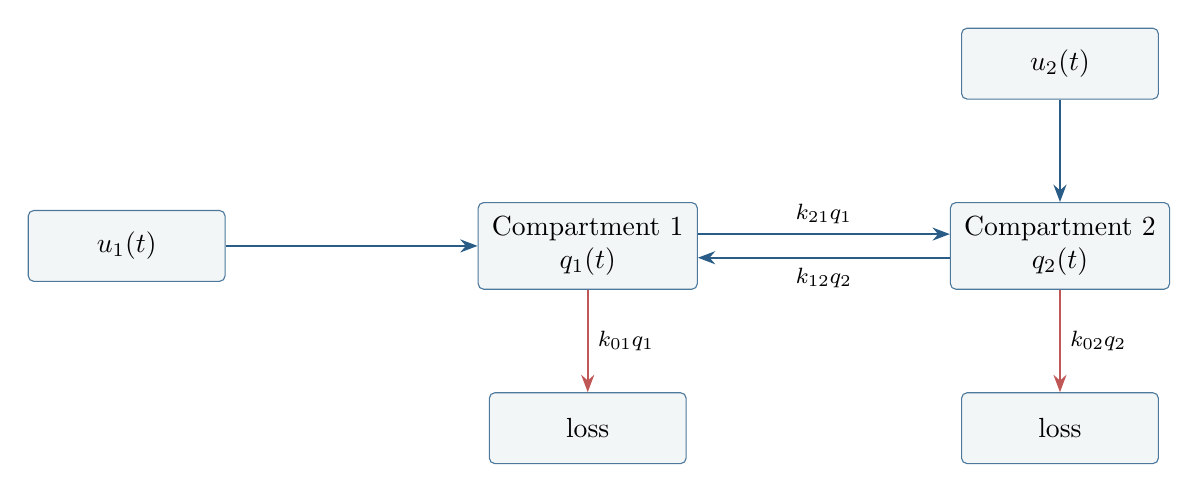
\begin{tikzpicture}[node distance=32mm]
  \node[comp] (u1) {\(u_1(t)\)};
  \node[comp, right=of u1] (c1) {Compartment 1\\\(\qone(t)\)};
  \node[comp, right=of c1] (c2) {Compartment 2\\\(\qtwo(t)\)};
  \node[comp, below=13mm of c1] (e1) {loss};
  \node[comp, below=13mm of c2] (e2) {loss};
  \node[comp, above=13mm of c2] (u2) {\(u_2(t)\)};
  \draw[flow] (u1) -- (c1);
  \draw[flow] (u2) -- (c2);
  \draw[flow] ([yshift=1.5mm]c1.east) -- node[above,info]{\(k_{21}\qone\)} ([yshift=1.5mm]c2.west);
  \draw[flow] ([yshift=-1.5mm]c2.west) -- node[below,info]{\(k_{12}\qtwo\)} ([yshift=-1.5mm]c1.east);
  \draw[loss] (c1) -- node[right,info]{\(k_{01}\qone\)} (e1);
  \draw[loss] (c2) -- node[right,info]{\(k_{02}\qtwo\)} (e2);
\end{tikzpicture}
}
\end{center}

\subsection{Equations}

Mass balance gives
\[
  \begin{aligned}
  \ddt \qone
  &=-(k_{01}+k_{21})\qone+k_{12}\qtwo+u_1(t),\\
  \ddt \qtwo
  &=k_{21}\qone-(k_{02}+k_{12})\qtwo+u_2(t).
  \end{aligned}
\]
In matrix form:
\[
  \ddt
  \begin{bmatrix}
  \qone\\
  \qtwo
  \end{bmatrix}
  =
  \underbrace{
  \begin{bmatrix}
  -(k_{01}+k_{21}) & k_{12}\\
  k_{21} & -(k_{02}+k_{12})
  \end{bmatrix}}_{\mat A}
  \begin{bmatrix}
  \qone\\
  \qtwo
  \end{bmatrix}
  +
  \begin{bmatrix}
  u_1\\
  u_2
  \end{bmatrix}.
\]

Notice the diagonal terms are negative sums of all first-order exits from that compartment. The off-diagonal terms are gains from the other compartment. This pattern generalizes to large compartmental systems.

\subsection{Two-compartment code as a sign audit}

The two-compartment live script is especially useful because each code line can be checked against one arrow in the diagram:
\begin{verbatim}
q1 = y(1);
q2 = y(2);
dq1dt = -(k01+k21)*q1 + k12*q2 + IR1;
dq2dt =  k21*q1 - (k02+k12)*q2 + IR2;
derivVector = [dq1dt,dq2dt]';
\end{verbatim}
The diagonal loss terms \(-(k_{01}+k_{21})q_1\) and \(-(k_{02}+k_{12})q_2\) are the easiest place to make a sign error. The transfer \(k_{21}q_1\) must appear once as a loss from compartment 1 and once as a gain to compartment 2. The transfer \(k_{12}q_2\) must do the opposite. In practice I would mark the diagram and code with the same colors before trusting a simulation.

The script's input reversal exercise is also a code-level identifiability lesson. Changing \code{IR1} and \code{IR2} changes which state receives external mass. If symmetric parameters and symmetric inputs make the curves overlap, the overlap is not a numerical accident; it is a structural property of the model.

\subsection{Steady state for the in-class parameters}

The live script uses
\[
  k_{01}=k_{02}=k_{12}=k_{21}=1,\qquad
  u_1=2,\qquad
  u_2=0.
\]
At steady state:
\[
  \begin{aligned}
  0&=-2\qone+\qtwo+2,\\
  0&=\qone-2\qtwo.
  \end{aligned}
\]
The second equation gives \(\qone=2\qtwo\). Substitution gives
\[
  -4\qtwo+\qtwo+2=0,
  \qquad
  \qtwo^*=\frac{2}{3},
  \qquad
  \qone^*=\frac{4}{3}.
\]
This is a useful check against the numerical simulation. If the plotted curves do not settle near these values, something is wrong in the code, parameter assignment, or interpretation of input direction.

\subsection{What reversing the input teaches}

The transcript notes that reversing the inputs reverses the curves, and equal inputs can make the two curves overlap under symmetric rates \cite{bmeg671TranscriptSep032025}. That observation is a gentle introduction to symmetry and identifiability. If two compartments have symmetric rates and the same input-output structure, they may become hard to distinguish from data. Model structure determines what can be learned.

\subsection{Output equations}

The two-compartment state is not automatically the measured data. If only compartment 1 is measured:
\[
  y(t)=
  \begin{bmatrix}1&0\end{bmatrix}
  \begin{bmatrix}\qone(t)\\ \qtwo(t)\end{bmatrix}.
\]
If concentration is measured, not amount:
\[
  y(t)=\frac{\qone(t)}{V_1}.
\]
If assay noise is present:
\[
  \tilde y_i = y(t_i)+\varepsilon_i,
  \qquad
  \varepsilon_i\sim\Normal(0,\sigma^2).
\]
This small output layer is the doorway from deterministic simulation to statistical inference.

\section{The Butyrate Translation Exercise}

\subsection{Why this example matters}

The lectures use a butyrate and bone-formation example drawn from the instructor's research area. Biologically, butyrate is a short-chain fatty acid produced by gut microbiota; experimental work such as Tyagi et al. links probiotic-induced butyrate increases to regulatory T cell expansion, WNT10B signaling, and bone formation \cite{tyagi2018butyrateBone}. The classroom task is not to reproduce the full biology. It is to practice translation:
\[
  \text{verbal pathway}
  \longrightarrow
  \text{compartment diagram}
  \longrightarrow
  \text{ODEs}.
\]

\subsection{A minimal two-state version}

Let \(\Bint(t)\) be butyrate amount in intestine and \(\Bblood(t)\) be butyrate amount in blood. Suppose butyrate is formed in intestine at rate \(F_{B1}\), exits intestine and blood with first-order rate \(\mu_B\), transfers from intestine to blood with rate constant \(A_{B12}\), and transfers from blood toward bone with rate constant \(A_{B23}\). If bone is treated as a downstream sink rather than a state, a minimal model is:
\[
  \begin{aligned}
  \ddt \Bint
  &=F_{B1}-(\mu_B+A_{B12})\Bint,\\
  \ddt \Bblood
  &=A_{B12}\Bint-(\mu_B+A_{B23})\Bblood.
  \end{aligned}
\]

\begin{center}
\resizebox{0.96\textwidth}{!}{%
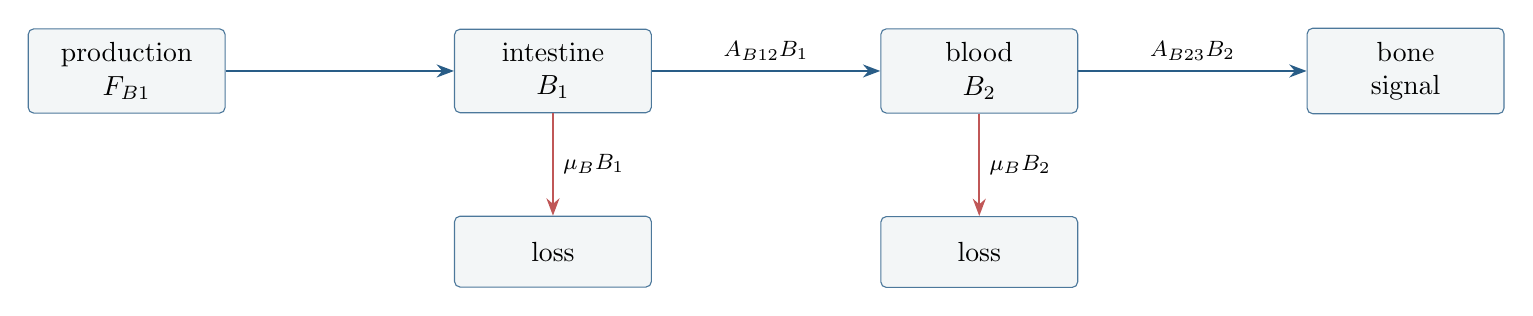
\begin{tikzpicture}[node distance=29mm]
  \node[comp] (prod) {production\\\(F_{B1}\)};
  \node[comp, right=of prod] (gut) {intestine\\\(\Bint\)};
  \node[comp, right=of gut] (blood) {blood\\\(\Bblood\)};
  \node[comp, right=of blood] (bone) {bone\\signal};
  \node[comp, below=13mm of gut] (eg) {loss};
  \node[comp, below=13mm of blood] (eb) {loss};
  \draw[flow] (prod) -- (gut);
  \draw[flow] (gut) -- node[above,info]{\(A_{B12}\Bint\)} (blood);
  \draw[flow] (blood) -- node[above,info]{\(A_{B23}\Bblood\)} (bone);
  \draw[loss] (gut) -- node[right,info]{\(\mu_B\Bint\)} (eg);
  \draw[loss] (blood) -- node[right,info]{\(\mu_B\Bblood\)} (eb);
\end{tikzpicture}
}
\end{center}

\subsection{Adding a bone state}

If bone exposure or effect is explicitly modeled, add a third state:
\[
  \ddt \Bone=A_{B23}\Bblood-k_{\mathrm{bone}}\Bone.
\]
This is a modeling choice. If the data include only gut and serum butyrate, a bone state may be weakly identifiable. If the data include bone biomarkers or bone formation rate, the bone state may be needed. This is exactly the kind of judgment the course wants students to develop.

\subsection{The key modeling lesson}

The butyrate example has a richer biological story than the one-compartment drug model, but the mathematical grammar is the same:
\[
  \text{formation}
  -
  \text{loss}
  -
  \text{transfer out}
  +
  \text{transfer in}.
\]
Once this grammar is internalized, many biomedical systems become approachable.

\section{Nonlinear Elimination}

\subsection{Why linearity breaks}

Lecture 3 introduces a nonlinear one-compartment model:
\[
  \ddt q(t)=\IRate-\frac{Cq(t)}{K+q(t)}.
\]
Here \(K\) has units of amount and controls the saturation scale; \(C\) has units of amount/time and controls the maximum elimination capacity \cite{bmeg671TranscriptSep032025}. This is Michaelis--Menten-like elimination written in amount units.

For small \(q\) relative to \(K\),
\[
  \frac{Cq}{K+q}
  \approx
  \frac{C}{K}q.
\]
So the system behaves approximately like a linear first-order elimination model with \(k=C/K\). For large \(q\),
\[
  \frac{Cq}{K+q}
  \approx C.
\]
The elimination rate saturates.

\subsection{Steady state condition}

At steady state:
\[
  \IRate=\frac{Cq^*}{K+q^*}.
\]
Solving:
\[
  \IRate(K+q^*)=Cq^*,
  \qquad
  \IRate K=(C-\IRate)q^*,
\]
so
\[
  q^*=\frac{\IRate K}{C-\IRate}.
\]
This exists as a positive finite steady state only when
\[
  \IRate<C.
\]
If input rate approaches capacity, \(q^*\) grows sharply. If input rate exceeds capacity, no finite steady state exists; the amount keeps rising. This is the mathematical version of the lecture's qualitative statement that high input can overwhelm elimination.

\subsection{Code scan for capacity stress testing}

The nonlinear live script turns the algebra into a stress test by changing the input rate while keeping \(C\) and \(K\) fixed \cite{bmeg671MatlabNonlinearStability2025}:
\begin{verbatim}
IRs = [0.01 0.02 1 2.5 5];
C = 1;
K = 1;

function derivVector = ODEs(t,y,IR,C,K)
  q = y(1);
  dqdt = IR - C*q/(K+q);
  derivVector = [dqdt]';
end
\end{verbatim}
The pedagogical point is that \code{IRs} is not just a plotting convenience. It asks whether the qualitative behavior is stable across experimental regimes. For \(\IRate<C\), trajectories can settle. For \(\IRate\ge C\), the code should show continued growth, because the modeled system has no finite positive steady state. If a numerical plot appears to ``plateau'' in that regime, it is a warning to inspect the time horizon, axis scaling, solver tolerances, or equation implementation.

\subsection{Why this matters pharmacologically}

Linear models are forgiving: doubling input doubles steady state. Saturable models are not. Near capacity, a small increase in dose can produce a large increase in exposure. This is why nonlinear elimination is not just a mathematical curiosity; it is a safety issue. Classic examples in pharmacokinetics include saturable metabolism, saturable transport, and target-mediated drug disposition.

\subsection{Local linearization}

Even nonlinear models can be studied locally. Let
\[
  f(q)=\IRate-\frac{Cq}{K+q}.
\]
Then
\[
  f'(q)=-\frac{CK}{(K+q)^2}.
\]
Near a steady state \(q^*\), perturbations \(\Delta q=q-q^*\) approximately satisfy
\[
  \ddt \Delta q
  \approx
  f'(q^*)\Delta q.
\]
Because \(f'(q^*)<0\), the steady state is locally stable when it exists. This tiny calculation is the bridge from nonlinear biological models to linear stability analysis later in the course.

\section{The SIR Model as a Compartmental Model}

\subsection{Equations}

The SIR model appears in Lecture 3 as another compartmental system:
\[
  \begin{aligned}
  \ddt S&=-\beta SI,\\
  \ddt I&=\beta SI-aI,\\
  \ddt R&=aI.
  \end{aligned}
\]
Here \(S\), \(I\), and \(R\) are susceptible, infected, and recovered populations or fractions. The infection term \(\beta SI\) is nonlinear because it depends on contact between susceptible and infected individuals.

\subsection{SIR code pattern}

The SIR live script uses the same state-vector grammar as the \PK{} scripts:
\begin{verbatim}
S = y(1);
I = y(2);
R = y(3);

dSdt = -beta*S*I;
dIdt =  beta*S*I - a*I;
dRdt =  a*I;
derivVector = [dSdt,dIdt,dRdt]';
\end{verbatim}
This is where code becomes a mass-balance proof. The term \(\beta SI\) disappears from \(S\) and appears in \(I\); the term \(aI\) disappears from \(I\) and appears in \(R\). Adding the three code lines should give zero, just as adding the equations gives conservation. A reader can therefore verify the script before thinking about epidemiology.

The code also makes the nonlinear leap visible. In the one-compartment model, every flow was proportional to one state. Here infection is proportional to a product of two states. That product is the doorway to thresholds, local linearization, and stability analysis in Module 2.

\subsection{Conservation}

Adding the equations gives
\[
  \ddt(S+I+R)=0.
\]
So \(S+I+R\) is conserved. If the initial values are fractions and sum to one, they remain fractions summing to one. This is the same conservation instinct as mass balance, now applied to population categories.

\subsection{Units}

If \(S\) and \(I\) are concentrations or population amounts, \(\beta\) must carry the reciprocal units needed to make \(\beta SI\) a rate. If \(S\) and \(I\) are fractions, units simplify. The transcript notes that biological modeling tools may require biological units rather than purely physical units \cite{bmeg671TranscriptSep032025}. This is not pedantry: units determine whether the model can be interpreted, shared, and checked.

\subsection{Why SIR belongs in this course}

At first, SIR may feel unrelated to drug distribution. But structurally it is the same kind of object:
\[
  \dot{\vect q}=f(\vect q,\vect\theta).
\]
The difference is that transfer from \(S\) to \(I\) depends on two states rather than one. This nonlinear interaction is a preview of immune response, tumor growth, virus-host dynamics, and many disease models.

\section{Verification, Validation, and Credibility}

\subsection{A practical distinction}

The first week gives a student-friendly distinction:
\begin{itemize}[leftmargin=2em]
  \item Verification asks: did we implement the intended equations correctly?
  \item Validation asks: do the intended equations adequately represent the real system for the intended use?
\end{itemize}
This distinction will become increasingly important as models become too complex for analytical solutions.

For the one-compartment impulse model, the analytical solution \(Q_0e^{-kt}\) is a verification oracle. For a butyrate or SIR model, the truth source may be experimental data, literature ranges, qualitative biological behavior, or independent simulations.

\subsection{ASME V and V 40}

ASME V\&V 40 frames credibility as evidence that a computational model is adequate for a specified context of use, with rigor commensurate with decision consequence \cite{asmeVV402018}. Although V\&V 40 was written for medical devices, the logic transfers well to biomedical and pharmaceutical modeling:
\[
  \text{more consequential model use}
  \quad\Rightarrow\quad
  \text{stronger credibility evidence needed}.
\]
A homework simulation needs clear equations and code checks. A dose-selection model affecting a clinical program needs documented assumptions, data provenance, sensitivity analysis, uncertainty analysis, external checks, and transparent communication of limitations.

\subsection{MIDD and the question of interest}

FDA's \MIDD{} paired meeting program and ICH M15 both formalize the idea that models can support drug development decisions when the model question, evidence, assumptions, and uncertainty are clear \cite{fdaMiddProgram2026,ichM15Midd2026}. The phrase ``question of interest'' is especially useful. A model should not be judged by whether it is complicated. It should be judged by whether it answers a specific question:
\[
  \text{Can this model support this decision under this uncertainty?}
\]

That question is already visible in the course's HW1 instructions. A chosen paper/model should have real measurements, a manageable ODE state dimension, and a scientifically meaningful comparison between model and data \cite{bmeg671Lecture2Slides2025,bmeg671TranscriptSep032025}.

\subsection{Model exchange and SBML}

As models grow, reproducibility becomes a real problem. \SBML{} is a community standard for representing systems biology models in machine-readable form \cite{sbmlLevel3Version2Release2}. Students do not need to master \SBML{} in week one, but they should understand the motivation: a model is more credible when its equations, parameters, units, compartments, species, and events are represented in a portable, inspectable form.

\section{Choosing a Course Project}

\subsection{The assignment logic}

Lecture 3 explains HW1 as the beginning of a semester-long modeling arc. The student chooses a biomedical or pharmaceutical ODE model, ideally with 3--10 states, real measurements for comparison, and a unique primary article \cite{bmeg671Lecture2Slides2025,bmeg671TranscriptSep032025}. This is not busywork. It is a way to make every later technique attach to one concrete system.

\subsection{Good project shapes}

Good early projects often have:
\begin{itemize}[leftmargin=2em]
  \item a clear compartment diagram;
  \item a small state vector;
  \item documented parameter values or estimable parameters;
  \item data over time, not merely endpoint data;
  \item one or two scientifically meaningful outputs;
  \item a reason to care about prediction or mechanism.
\end{itemize}

Examples include a simple \PKPD{} model, a tumor growth inhibition model, a viral dynamics model, an immune response model, a glucose-insulin model, a bone remodeling model, or a reduced \QSP{} module.

\subsection{Warning signs}

Warning signs include:
\begin{itemize}[leftmargin=2em]
  \item a model with dozens of states before the student knows what each state means;
  \item no available time-course data;
  \item parameters copied without units;
  \item a diagram that cannot be translated into equations;
  \item equations with terms that do not share units;
  \item a project question that is too broad, such as ``model cancer.''
\end{itemize}

The best project question is narrow enough to simulate and broad enough to matter:
\[
  \text{How does changing this rate or input alter this observable time course?}
\]

\section{A Study Checklist for the First Three Lectures}

\subsection{Before writing equations}

Ask:
\begin{itemize}[leftmargin=2em]
  \item What is the biological or pharmaceutical story?
  \item What are the compartments?
  \item What species is tracked in each compartment?
  \item Are states amounts, concentrations, fractions, or counts?
  \item Which arrows are transfers, which are reactions, which are external inputs, and which are losses?
  \item What is measured?
\end{itemize}

\subsection{While writing equations}

Check:
\begin{itemize}[leftmargin=2em]
  \item each inflow appears with a plus sign;
  \item each outflow appears with a minus sign;
  \item each internal transfer appears in two equations with opposite signs;
  \item every term in a differential equation has the same units;
  \item input type matches experiment: impulse, step, or time-varying;
  \item initial conditions match the protocol.
\end{itemize}

\subsection{After coding}

Verify:
\begin{itemize}[leftmargin=2em]
  \item known analytical solutions are reproduced;
  \item mass conservation holds when it should;
  \item steady states match algebraic calculations;
  \item curves have biologically plausible signs and magnitudes;
  \item solver choices and tolerances do not change conclusions unexpectedly;
  \item plotted outputs correspond to measured quantities, not merely hidden states.
\end{itemize}

\subsection{Before believing the model}

Validate:
\begin{itemize}[leftmargin=2em]
  \item compare predictions with data not used only for coding checks;
  \item inspect residuals or systematic deviations;
  \item ask whether the model answers the intended question;
  \item state which mechanisms are included and which are deliberately lumped;
  \item communicate uncertainty and limitations.
\end{itemize}

\section{Worked Micro-Examples}

\subsection{Example 1: a urinary excretion accounting state}

Suppose a drug amount \(q_c\) is in central compartment and cumulative urinary amount is \(q_u\). Let renal excretion be \(k_rq_c\) and nonrenal elimination be \(k_nq_c\):
\[
  \begin{aligned}
  \dot q_c&=u(t)-(k_r+k_n)q_c,\\
  \dot q_u&=k_rq_c.
  \end{aligned}
\]
The urinary state has no loss because it is cumulative collected amount. If the experiment measures urine over intervals, the observable is not \(q_u(t_i)\) itself but increments:
\[
  \Delta q_{u,i}=q_u(t_i)-q_u(t_{i-1}).
\]
This small detail matters for fitting.

\subsection{Example 2: a reversible distribution state}

For central \(q_c\) and tissue \(q_t\):
\[
  \begin{aligned}
  \dot q_c&=u(t)-k_{ct}q_c+k_{tc}q_t-k_{\mathrm{el}}q_c,\\
  \dot q_t&=k_{ct}q_c-k_{tc}q_t.
  \end{aligned}
\]
Here the tissue state is not cumulative. It can fill and empty. The transfer terms appear with opposite signs. If only central concentration is measured, the tissue state is hidden but may be inferred indirectly from the curve shape.

\subsection{Example 3: a simple effect compartment}

If plasma concentration \(C_p\) changes faster than effect-site concentration \(C_e\), introduce:
\[
  \dot C_e=k_{e0}(C_p-C_e).
\]
This equation says the effect site relaxes toward plasma with rate \(k_{e0}\). A direct effect model might use \(E(t)=E_{\max}C_p/(EC_{50}+C_p)\). An effect-compartment model uses:
\[
  E(t)=\frac{E_{\max}C_e(t)}{EC_{50}+C_e(t)}.
\]
This is a preview of later \PKPD{}: delays often mean a missing state or a missing turnover process.

\section{Summary}

\subsection{One paragraph}

The first three BMEG 671 meetings teach a modeling language rather than a list of equations. A compartment is a deliberate abstraction; a state is the quantity that changes; an input encodes the experimental protocol; an output connects hidden dynamics to measurements. Mass balance turns diagrams into ODEs. Step and impulse inputs distinguish sustained supply from instantaneous dosing. One-compartment models teach exponential decay, steady state, and code verification. Two-compartment models teach matrix form, transfer signs, symmetry, and output maps. Butyrate and SIR examples show that the same grammar scales from \PK{} to microbiome-bone biology and infectious disease. Nonlinear elimination shows why saturation changes qualitative behavior. Verification checks whether the equations and code match; validation asks whether the model is adequate for a question. This is the foundation on which the rest of the course will build controllability, observability, identifiability, estimation, uncertainty, and model selection.

\subsection{The sentence to keep}

For any new biomedical model, ask:
\begin{center}
\fbox{\parbox{0.88\textwidth}{\centering What are the states, what moves between them, what is measured, and what decision will this model support?}}
\end{center}
If that sentence is clear, the mathematics has a place to stand.

\bibliographystyle{plain}
\bibliography{../refs/pharmacology}

\end{document}
